\begin{figure}
\centering
\small
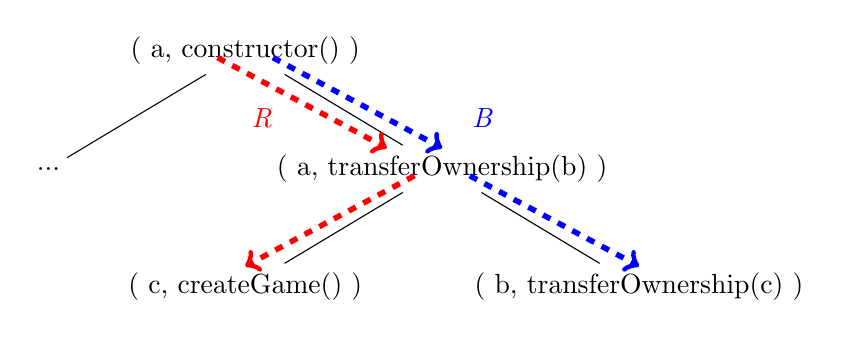
\begin{tikzpicture}
	\node (root) {( a, constructor() )}
	[sibling distance=50mm]
	child {node {...}}
	child {node (transfer1) {( a, transferOwnership(b) )}
		child {node (create) {( c, createGame() )}}
		child {node (transfer2) {( b, transferOwnership(c) )}}
	};
%	\draw [line width=3pt, red] ([yshift=10pt, xshift=-5pt]root.base) -- ([yshift=-10pt, xshift=-5pt]transfer1.base) -- (create.base) ;

	\path [line width=2pt, ->, dashed, blue] ([ xshift=10pt]root.base) edge ([ yshift=10pt]transfer1.base);
	\path [line width=2pt, ->, dashed, blue] ([ xshift=10pt]transfer1.base) edge ([ yshift=10pt]transfer2.base) ;
	
	\path [line width=2pt, ->, dashed, red] ([ xshift=-10pt]root.base) edge ([ yshift=10pt, xshift=-20pt]transfer1.base);
	\path [line width=2pt, ->, dashed, red] ([ xshift=-10pt,]transfer1.base) edge ([ yshift=10pt]create.base) ;
	
	\draw ([xshift=15pt, yshift=10pt]transfer1.north) node[] {\textcolor{blue}{\textit{B}}} ;
	
	\draw ([xshift=-65pt, yshift=10pt]transfer1.north) node[] {\textcolor{red}{\textit{R}}} ;
	
\end{tikzpicture}
\caption{Execution tree of Dicether}
\label{fig: HyperLTLfailure}
\end{figure}